\documentclass{standalone}
\usepackage{pgfplots}
\begin{document}
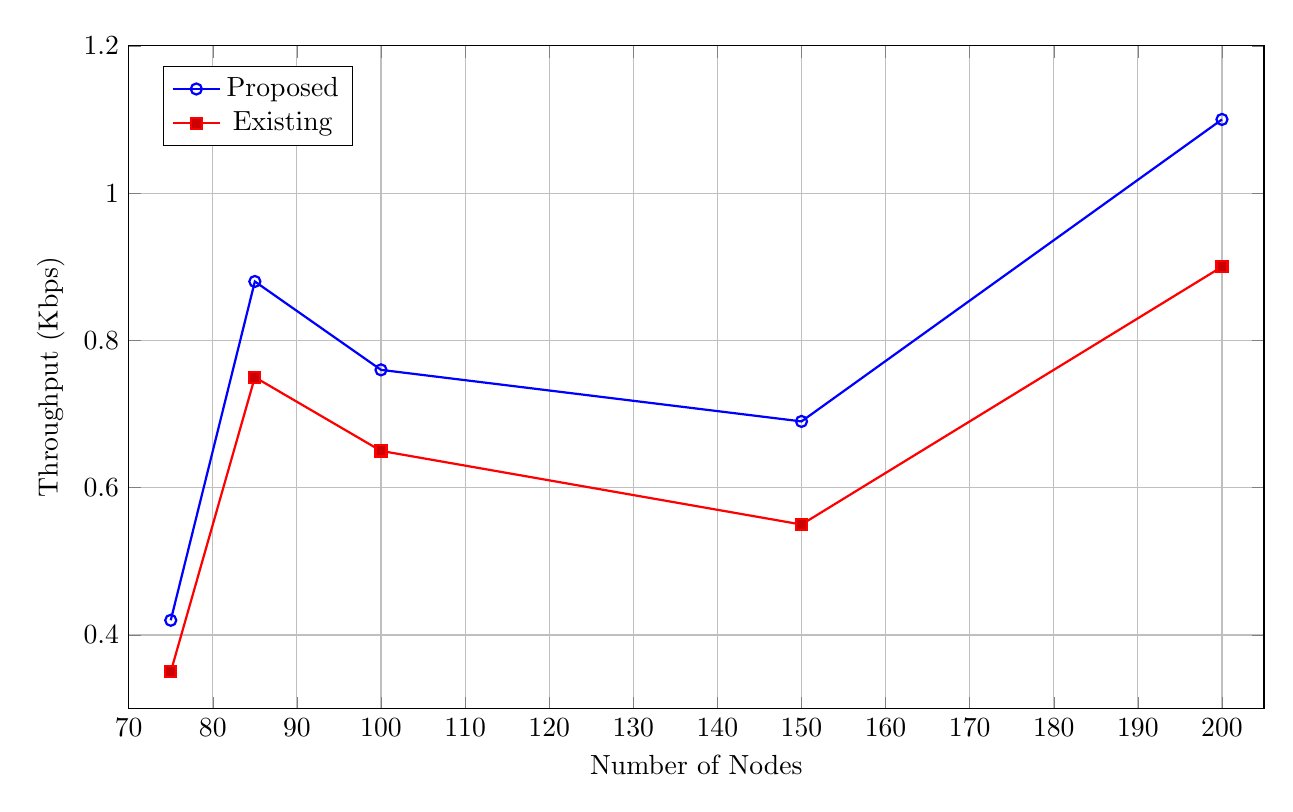
\begin{tikzpicture}
\begin{axis}[
width=16cm,height=10cm,
xlabel={Number of Nodes},
ylabel={Throughput (Kbps)},
xmin=70,xmax=205,
ymin=0.3,ymax=1.2,
grid=major,
legend pos=north west
]
\addplot+[mark=o,thick] coordinates {
(75,0.42)(85,0.88)(100,0.76)(150,0.69)(200,1.10)
};
\addplot+[mark=square*,thick] coordinates {
(75,0.35)(85,0.75)(100,0.65)(150,0.55)(200,0.90)
};
\legend{Proposed,Existing}
\end{axis}
\end{tikzpicture}
\end{document}